\documentclass[cal1spr16Lectures.tex]{subfiles}

\begin{document}

%\section[Week 12]{Week 12: 11-15 Apr}

% % % 
\subsubsection{\bf Wednesday 13 April}
% % %

\begin{frame}[allowframebreaks]{Wed 13 Apr}
\begin{itemize}\footnotesize
\item Exam 3

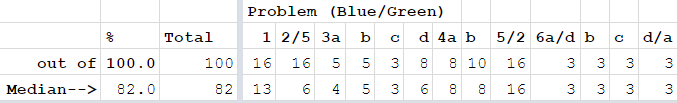
\includegraphics[scale=0.5]{../Exam3Medians}

Spread:

\begin{center}
\includegraphics[scale=0.5]{../Exam3Spread}
\end{center}
\item No (scheduled) office hours today.  I will be in \~1220p.
\item ALL MLPs are open now.
\item April 22: Last day to drop with a "W".
\end{itemize}
\end{frame}

% % %
\subsubsection{Examining Growth Rates}
% % %

% % %
\begin{frame}{\small Examining Growth Rates}\footnotesize
We can use l'H\^{o}pital's Rule to examine the rate at which functions grow in comparison to one another.
\begin{dfn} Suppose $f$ and $g$ are functions with $\displaystyle\lim_{x \to \infty} f(x) = \displaystyle\lim_{x \to \infty} g(x) = \infty$.  Then $\boldsymbol{f}$ {\bf grows faster than} $\boldsymbol{g}$ as $x \to \infty$ if 
$$\lim_{x \to \infty} \frac{g(x)}{f(x)} = 0\ \text{or}\ \lim_{x \to \infty} \frac{f(x)}{g(x)} = \infty.$$
$g \ll f$ means that $f$ grows faster than $g$ as $x \to \infty$.
\end{dfn}

\begin{dfn} The functions $f$ and $g$ have {\bf comparable growth rates} if 
$$\lim_{x \to \infty} \frac{f(x)}{g(x)}=M,\ \text{where}\ 0<M<\infty.$$
\end{dfn}
\end{frame}

% % %
\subsubsection{Pitfalls in Using L\^opital's Rule}
% % %

% % %
\begin{frame}{\small Pitfalls in Using l'H\^{o}pital's Rule}
\footnotesize
\begin{itemize}
\item[1.] L'H\^{o}pital's Rule says that $\displaystyle\lim_{x \to a}\frac{f(x)}{g(x)} = 
\displaystyle\lim_{x \to a}\frac{f^{\prime}(x)}{g^{\prime}(x)}$.  \alert{NOT} 
\[\lim_{x \to a}\frac{f(x)}{g(x)} = \lim_{x \to a}\left[ \frac{f(x)}{g(x)} \right]^{\prime}\ \text{or}\
\lim_{x \to a}\frac{f(x)}{g(x)} = \lim_{x \to a} \left[ \frac{1}{g(x)} \right]^{\prime} f^{\prime}(x)\]
(i.e., don't confuse this rule with the Quotient Rule).
\item[2.] Be sure that the limit with which you are working is in the form $\frac{0}{0}$ or $\frac{\infty}{\infty}$.
\item[3.] When using l'H\^{o}pital's Rule more than once, simplify as much as possible before repeating the rule.
\item[4.] If you continue to use l'H\^{o}pital's Rule in an unending cycle, another method must be used.
\end{itemize}
\end{frame}

% % %
\subsubsection{Book Problems}
% % %

% % % 
\begin{frame}
\begin{block}{4.7 Book Problems}
13-59 (odds), 69-79 (odds)
\end{block}
\end{frame}

% % %
\subsection[4.9 Antiderivatives]{\S 4.9 Antiderivatives}\small
% % %

% % %
\begin{frame}{\S 4.9 Antiderivatives}\small
With differentiation, the goal of problems was to find the function $f^{\prime}$ given the function $f$.

\vspace{1pc}
With antidifferentiation, the goal is the opposite.  Here, given a function $f$, we wish to find a function $F$ such that the derivative of $F$ is the given function $f$ (i.e., $F^{\prime}=f$).
\end{frame}

% % %
\begin{frame}\small
\begin{dfn} A function $F$ is called an {\bf antiderivative} of a function $f$ on an interval $I$ provided $F^{\prime}(x)=f(x)$ for all $x$ in $I$. \end{dfn}

\vspace{1pc}
\begin{ex} Given $f(x)=4$, an antiderivative of $f(x)$ is $F(x)=4x$.  \end{ex}

NOTE: Antiderivatives are not unique!
\end{frame}

% % %
\begin{frame}\footnotesize
They differ by a constant ($C$):

\begin{thm}
Let $F$ be any antiderivative of $f$.  Then {\bf all} the antiderivatives of $f$ have the form $F+C$, where $C$ is an arbitrary constant.
\end{thm}

\vspace{1pc}
{\bf Recall:} $\dfrac{d}{dx} f(x)=f'(x)$ is the derivative of $f(x)$. 

\vspace{1pc}
{\bf Now:} $\int f(x)\ dx=F+C$ \alert{\it is} the antiderivative of $f(x)$.  It doesn't matter which $F$ you choose, since writing the $C$ will show you are talking about all the antiderivatives at once.  The $C$ is also why we call it the {\it indefinite} integral.
\end{frame}

% % %
\begin{frame}
\begin{ex}
Find the antiderivatives of the following functions:
\begin{itemize}
\item[(1) ]$f(x)=-6x^{-7}$
\item[(2) ]$g(x)=-4\cos{4x}$
\item[(3) ]$h(x)=\csc^2{x}$
\end{itemize}
\end{ex}
\end{frame}

% % %
\subsubsection{Indefinite Integrals}
% % %

% % %
\begin{frame}{\small Indefinite Integrals}\small
\begin{ex} $\int 4x^3\ dx = x^4+C$, where $C$ is the {\bf constant of integration}. \end{ex}

\vspace{1pc}
The $dx$ is called the {\bf differential} and it is the same $dx$ from Section 4.5.  Like the $\frac{d}{dx}$, it shows which variable you are talking about.  The function written between the $\int$ and the $dx$ is called the {\bf integrand}.
\end{frame}

% % %
\subsubsection{Rules for Indefinite Integrals}
% % %

% % %
\begin{frame}{\small Rules for Indefinite Integrals}\footnotesize
{\bf Power Rule:}  $\int x^p\ dx = \dfrac{x^{p+1}}{p+1} + C$ 

\vspace{0.65pc}
\hspace{5ex}($p$ is any real number except $-1$) 

\vspace{1.5pc}
{\bf Constant Multiple Rule:} $\int c f(x)\ dx = c \int f(x)\ dx$

\vspace{1.5pc}
{\bf Sum Rule:} $\int \left(f(x)+g(x) \right)\ dx = \int f(x)\ dx + \int g(x)\ dx$
\end{frame}

% % %
\begin{frame}
\begin{exe}
\[\int(5x^4+2x+1)\ dx=\]
\begin{itemize}
\item[A. ] $20x^3+2+C$
\item[B. ] $x^5+x^2-x+C$
\item[C. ] $x^5+x^2+C$
\item[D. ] $x^5+2x^2-x+C$
\end{itemize}
\end{exe}
\end{frame}

% % %
\begin{frame}
\begin{exe} Evaluate the following indefinite integrals:
\begin{itemize}
\item[(1) ] $\int \left( 3x^{-2}-4x^2+1 \right)\ dx$
\item[(2) ] $\int 6 \sqrt[3]{x}\ dx$
\item[(3) ] $\int 2 \cos{(2x)}\ dx$
\end{itemize}
\end{exe}
\end{frame}

% % %
\subsubsection{Indefinite Integrals of Trig Functions}
% % %

% % %
\begin{frame}{\small Indefinite Integrals of Trig Functions}\footnotesize
Table 4.9 (p.\ 322) provides us with rules for finding indefinite integrals of trig functions.
\begin{alignat*}{4}
1.\ &\dfrac{d}{dx} (\sin ax) = a\cos ax &\longrightarrow &\int \cos ax\ dx = \dfrac{1}{a} \sin ax + C \\
2.\ &\dfrac{d}{dx} (\cos ax) = -a\sin ax &\longrightarrow &\int \sin ax\ dx = -\dfrac{1}{a} \cos ax + C \\
3.\ &\dfrac{d}{dx} (\tan ax) = a\sec^2 ax &\longrightarrow &\int \sec^2 ax\ dx = \dfrac{1}{a} \tan ax + C \\
4.\ &\dfrac{d}{dx} (\cot ax) = -a\csc^2 ax &\longrightarrow &\int \csc^2 ax\ dx = -\dfrac{1}{a} \cot ax + C \\
5.\ &\dfrac{d}{dx} (\sec ax) = a\sec ax \tan ax &\longrightarrow &\int \sec ax \tan ax\ dx = \dfrac{1}{a} \sec ax + C \\
6.\ &\dfrac{d}{dx} (\csc ax) = -a\csc ax \cot ax \ &\longrightarrow &\int \csc ax \cot ax\ dx = -\dfrac{1}{a} \csc ax + C
\end{alignat*}
\end{frame}

% % %
\begin{frame}\footnotesize
\begin{ex} 
Evaluate the following indefinite integral: $\int 2 \sec^2 2x\ dx$. 
\end{ex}

\vspace{1pc}
{\bf Solution:}  Using rule 3, with $a=2$, we have
\[\int 2 \sec^2 2x\ dx = 2 \int \sec^2 2x\ dx = 2 \left[ \dfrac{1}{2} \tan 2x \right] + C = \tan 2x + C.\]

\vspace{1pc}
\begin{exe} 
Evaluate $\int 2 \cos(2x)\ dx$. 
\end{exe}
\end{frame}

% % %
\subsubsection{Other Indefinite Integrals}
% % %

% % %
\begin{frame}{\small Other Indefinite Integrals}\footnotesize
%Table 4.6 (p.\ 297) provides us with rules for finding other indefinite integrals.
\begin{alignat*}{4}
7.\ &\dfrac{d}{dx} (e^{ax}) = a e^{ax} &\longrightarrow &\int e^{ax}\ dx = \dfrac{1}{a} e^{ax} + C \\
8.\ &\dfrac{d}{dx} (\ln |x|) = \dfrac{1}{x} &\longrightarrow &\int \dfrac{dx}{x} = \ln |x| + C \\
9.\ &\dfrac{d}{dx} \left( \sin^{-1} \left( \dfrac{x}{a} \right) \right) = \dfrac{1}{\sqrt{a^2-x^2}} &\longrightarrow 
&\int \dfrac{dx}{\sqrt{a^2-x^2}} = \sin^{-1} \left( \dfrac{x}{a} \right) + C \\
10.\ &\dfrac{d}{dx} \left( \tan^{-1} \left( \dfrac{x}{a} \right) \right) = \dfrac{a}{a^2+x^2} &\longrightarrow 
&\int \dfrac{dx}{a^2+x^2} = \dfrac{1}{a} \tan^{-1} \left( \dfrac{x}{a} \right) + C \\
11.\ &\dfrac{d}{dx} \left( \sec^{-1} \left| \dfrac{x}{a} \right| \right) = \dfrac{a}{x \sqrt{x^2-a^2}} &\longrightarrow 
&\int \dfrac{dx}{x \sqrt{x^2-a^2}} = \dfrac{1}{a} \sec^{-1} \left| \dfrac{x}{a} \right| + C
\end{alignat*}
\end{frame}

\end{document}